\chapter{Zahlenbereiche}
\section{Natürliche Zahlen}
Die natürlichen Zahlen 1, 2, 3, 4, \ldots ~sind die ältesten Zahlen, die sich aus dem Zählen von Gegenständen entwickelt haben.
Dabei nimmt man an, dass man immer weiterzählen kann.\\

\begin{defn}{Natürliche Zahlen}
	Die Menge der natürlichen Zahlen wird mit $\N$ bezeichnet.
	Man schreibt:
	\begin{align*} 
	 \N = \{ 1, 2, 3, 4, \ldots \}\, .
	\end{align*}
	Die Zahlen $1, 2, 3, 4, \ldots$ heissen \emph{Elemente} der Menge $\N$.
	Ist eine Zahl $n$ eine natürliche Zahl, so schreibt man: $n\in\N$\,.
\end{defn}

\vspace{.5cm}
\begin{wrapfigure}{r}{6cm}
	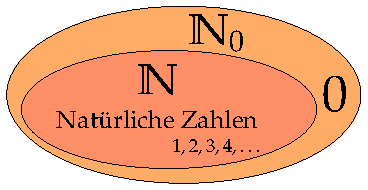
\includegraphics[width=\linewidth]{numberset-naturals-N0}
\end{wrapfigure}
Das Zeichen \glqq $\in$\grqq~bedeutet: \glqq ist Element von\grqq, das Zeichen \glqq $\notin$\grqq~bedeutet: \glqq ist \emph{nicht} Element von\grqq.

\paragraph{Achtung!}
Die Zahl 0 wird dabei {\bfseries nicht} mit dazu genommen.
Wir schreiben:
\begin{align*}
  0 \notin \N\, .
\end{align*}
Möchte man die Null mit einschliessen, so verwenden wir die Schreibweise $\N_0$.\\

\begin{defn}{Natürliche Zahlen zusammen mit Null}
	Die Menge der natürlichen Zahlen wird mit $\N_0$ bezeichnet.
	Man schreibt: $\N_0 = \{ 0, 1, 2, 3, 4, \ldots \}$\,.
\end{defn}

\begin{example}
  Schreibe in das Symbol \relationBox das richtige Zeichen $\in$ oder $\notin$ hinein.
  \begin{align*}
   2 \relationBox \N_0\,,\qquad
   \frac{1}{2} \relationBox \N\,,\qquad
   0 \relationBox \N\,,\qquad
   0 \relationBox \N_0\,,\qquad
   \frac{72}{36} \relationBox \N\,.
  \end{align*}

\end{example}


\vspace{.5cm}
Die natürlichen Zahlen braucht man z.B. um Anzahlen anzugeben, Rangplätze oder Reihenfolgen festzulegen oder (bestimmte) Messergebnisse festzuhalten.

\begin{example}~
	\begin{itemize}\setlength\itemsep{0pt}
		\item Wir haben heute 6 Lektionen. (Anzahl)
		\item Heute ist der erste Tag des Monats. (Rangplatz)
		\item Heute ist es 30 Grad warm. (Messergebnis)
	\end{itemize}
\end{example}

Man kann mit den natürlichen Zahlen auch (bestimmte) Gleichungen lösen.
\begin{example}
 Heute ist es 30 Grad warm und damit 2 Grad wärmer als gestern.
 D.h. für die Temperatur $x$ von gestern in Grad gilt die Gleichung:
 \begin{align*}
   x + 2 = 30
 \end{align*}
Die Lösung der Gleichung ist eine natürliche Zahl, nämlich $x = 28$.
\end{example}

\section{Ganze Zahlen}
\section{Rationale Zahlen}
\section{Kann man alle Zahlen als Bruch darstellen?}
% Hier muss noch etwas Geschichte hin.

